\chapter{Java Management Extensions}
\label{ch:4}
\textit{Java Management Extensions} (JMX) é uma API que fornece uma maneira simples e padrão de gestão e monitoramento de recursos para a plataforma Java. Estes recursos podem ser aplicações, dispositivos, serviços ou a própria JVM (\textit{Java Virtual Machine}). São instrumentados por um ou mais \textit{Managed Beans}, ou simplemente Mbeans, resposáveis por adquir, manipular ou enviar informações sobre o recurso~\cite{lindfors2002jmx}.

Essa tecnologia foi desenvolvida através do JCP (\textit{Java Community Process}), em duas JSRs (\textit{Java Specification Request}) distintas. A JSR 3, \textit{Java Management Extensions Instrumentation and Agent Specification} e a JSR 160, \textit{Java Management Extensions Remote API}.

JCP é o processo de desenvolvimento padrão de novas especificações para a plataforma Java, as chamadas JRSs, que são documentos que descrevem as especificações e tecnologias propostas à plataforma.

A especificação de JMX define, além da arquitetura, padrões de projeto, API's e um conjunto de serviços de gerenciamento e monitoramento. Possibilitando o desenvolvimento de aplicações gerenciáveis local ou remotamente através do processo de instrumentação, onde atributos, configurações e capacidades da aplicação são expostos. Aumentando a robustez e extensibilidade da aplicação, uma vez que, é possível construir soluções de gerenciamento inteligentes, interoperáveis e independentes da infra-estrutura de gestão~\cite{jmx}.
\newpage

\section{Arquitetura}

A arquitetura JMX é definida em três níveis, ver Figura \ref{fig:arch_jmx}:

\begin{itemize}
 \item Nível de Instrumentação;
 \item Nível de Agente;
 \item Nível de Gerenciamento.
\end{itemize}

Como foi dito anteriormente, JMX foi definida segundo duas JSRs , JSR 3 e JSR 160. Os dois primeiros níveis da arquitetura (Intrumentação e Agente) foram definidos na JSR 3, enquanto o Nível de Gerenciamento foi definido na JSR 160. Isso mostra, de certa forma, o pontencial de extensibilidade da tecnologia.
\newline

\begin{figure}[htp]
\centering
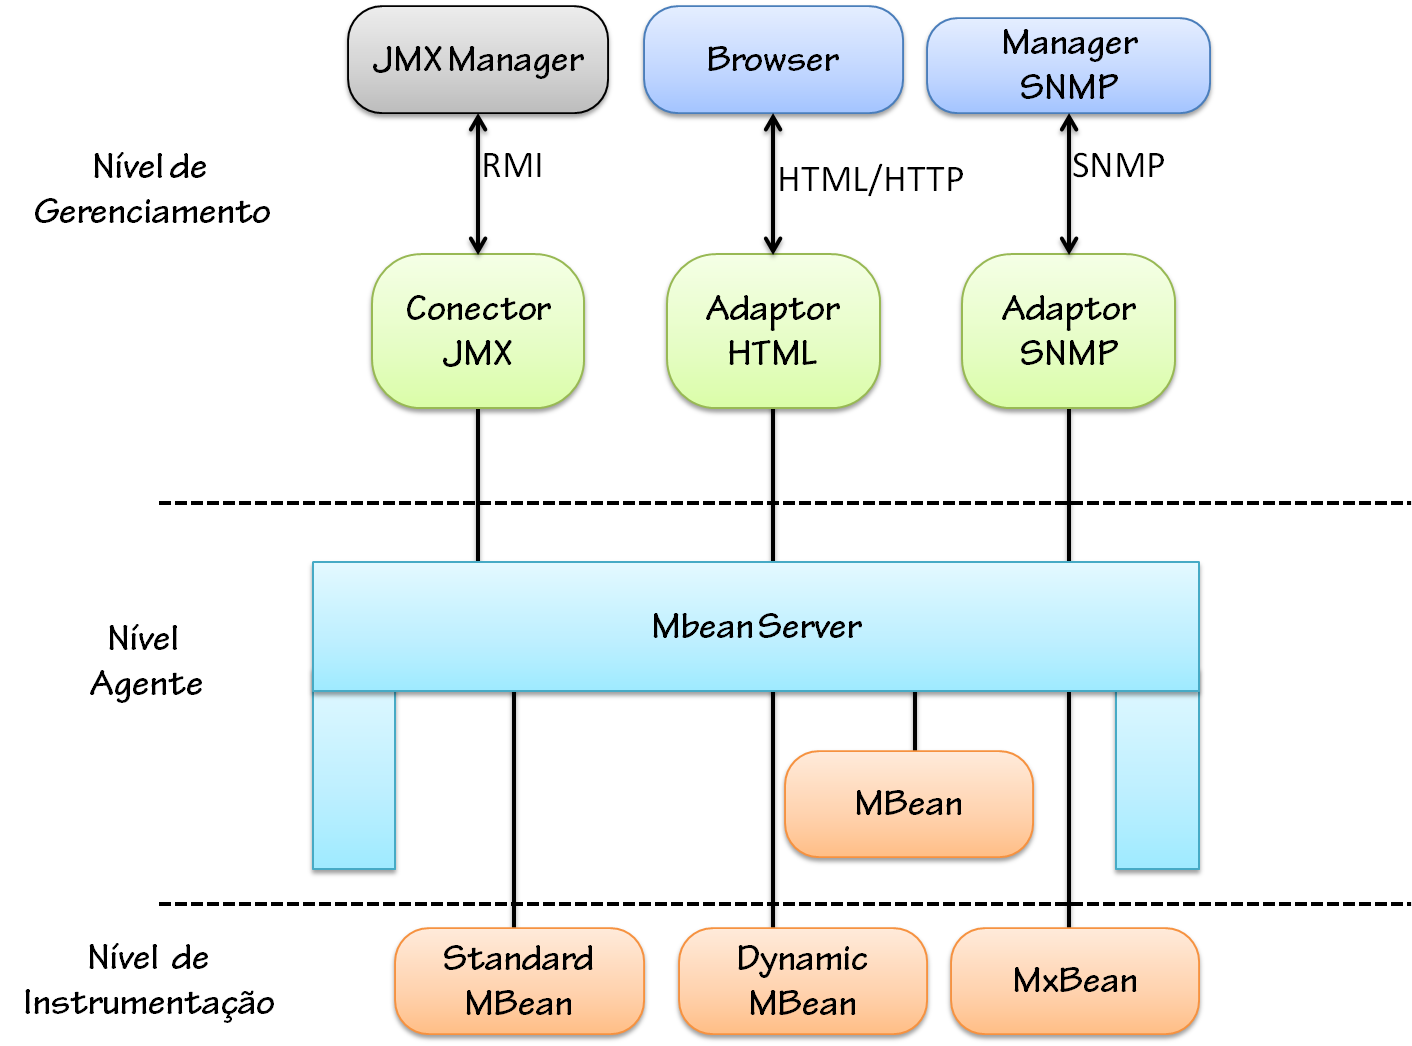
\includegraphics[width=12cm]{chapters/chapter4/arch_jmx.png}
\caption[Arquitetura JMX]{Arquitetura JMX.}
\label{fig:arch_jmx}
\end{figure}

\subsection{Nível de Intrumentação}
O nível de instrumentação é resposável por expor as funcionalidades e configurações das aplicações através da criação e registro de Mbeans~\cite{jmx}. Estes Mbeans coletam e manipulam as informações dos recursos gerenciáveis, repassando-as aos agentes JMX do nível superior.

\subsection{Nível Agente}
O nível agente é responsável por gerenciar todas as e controlar diretamente todos os recursos, tornando-os acessíveis a aplicativos de gerenciamento remoto.

A gerência das Mbeans é provida através do principal componente do agente JMX, o Mbean Server. Além disso, agentes JMX incluem um conjunto de serviços para gerenciar as MBeans e pelo menos um adaptador de comunicações ou conector para permitir o acesso ao agente por um aplicativo de gerenciamento~\cite{jmx}.

Basicamente, um agente JMX consiste em um Mbean Server, um conjunto de serviços básicos de gerência e pelo menos um adaptador de comunicação ou conector JMX.

\subsection{Nível de Gerenciamento}
O nível de gerenciamento é o nível mais alto da arquitetura JMX, este define um mecanismo baseado em adaptadores e conectores que tornam os agente JMX acessíveis a aplicativos de gerenciamento remoto fora da JVM em que o agente se encontra~\cite{jmx}.

Define de certa forma uma interface de acesso aos agentes JMX ao mundo externo, através de protocolos proprietários ou existentes (\textit{e.g.} SNMP - \textit{Simple Network Manager Protocol}, um protocolo padrão para gerenciamento de componetes de rede).

\section{Mecanismo Notificações}
Além dos três níveis de arquitetura, JMX provê um mecanismo de notificação que permite que aplicações ou Mbeans recebam eventos ou notificações com informações sobre o estado dos recursos gerenciados, podendo gerar estatísticas ou mesmo processar eventos relacionados ao funcionamento dos recursos~\cite{lindfors2002jmx}.

O modelo de notificação JMX é semelhante ao mecamismo de notificações de java, que define \textit{object listers} (recebem as notificações) registados a Mbean que envia as notificações \textit{(broadcaster Mbeans)}. A \textit{broadcaster Mbeans} envia eventos de notificação a todos os \textit{listeners} registrados~\cite{lindfors2002jmx}.

\newpage
\subsection{Componentes do Mecanismo de Notificações}

O mecanismo de notificações JMX possui os seguintes componentes:

\begin{center}
\begin{table*}[h]
\begin{supertabular}[]{|l|l|}
\hline
\textbf{Componente} & \textbf{Descrição}\\\hline
Notification & Representa um tipo genérico de notificação\\\hline
NotificationListener & Interface que permite o recebimento de notificações\\\hline
\multirow{2}{*}{NotificationFilter} & Interface que permite a filtragem de notificações. Assim, apenas\\ 
& notificações relevantes ao Listener são recebidas\\\hline
\multirow{2}{*}{NotificationBroradcaster} & Interface que permite que notificações sejam enviadas aos\\
& listeners registrados \\\hline
\end{supertabular}
\caption{Componentes do Mecanismo de Notificação}
\end{table*}
\end{center}

\subsection{Modelo de Notificação JMX}

TODO: FIGURA

\subsubsection{Funcionamento} 
\begin{enumerate}
\item MBean consumidor registra-se através da interface \textit{NotificationBroadcaster}

\item Mbean gerador emite uma notificação

\item A notificação é enviada aos Mbeans registrados

\item O Mbean consumidor recebe e filtra as notificações

\item As notificações não descartadas são tradatas
\end{enumerate}

\section{Componetes JMX}